\documentclass[parskip=full,11pt]{scrartcl}
\usepackage[utf8]{inputenc}

\title{Performance Dashboard for Continuous Benchmarking of HPC Libraries}
\author{Chingun Ariunbat, Jamil Bagga, Walter Alexander B\"ottcher,\\Darius Schefer, Maximilian Schik}

% section numbers in margins:
\renewcommand\sectionlinesformat[4]{\makebox[0pt][r]{#3}#4}

\newcommand{\scenario}[2]{\textbf{Scenario name:} #1 \\
\textbf{Participating actor:} #2}

\newcommand{\case}[6]{\textbf{Use case name:} #1 \\
\textbf{Participating actors:} #2 \\
\textbf{Entry conditions:} #3 \\
\textbf{Flow of events:} #4 
\textbf{Exit conditions:} #5 \\
\textbf{Quality requirements:} #6
}

% header & footer
\usepackage{scrlayer-scrpage}
%\lofoot{\today} % Date in footer
\refoot{\today}  % no idea what this does
\pagestyle{scrheadings}

\usepackage[sfdefault,light]{roboto}
\usepackage[T1]{fontenc}
\usepackage[english]{babel}
\usepackage[yyyymmdd]{datetime} % must be after babel
\renewcommand{\dateseparator}{-}
\usepackage[colorlinks=true, linkcolor=blue]{hyperref}
\usepackage{amsmath} % for $\text{}$
\usepackage[nameinlink]{cleveref}
\crefname{figure}{Abb}{Abb}
\usepackage[section]{placeins}
\usepackage{xcolor}
\usepackage[nonumberlist, toc]{glossaries}     % provides glossary commands, [toc] to appear in table of contents
\usepackage{graphicx}
\graphicspath{ {./images/} }
\hypersetup{
	pdftitle={Specification},
	bookmarks=true,
}
\usepackage{csquotes} % provides \enquote{} command
\usepackage{specification}

\makenoidxglossaries

\newglossaryentry{developer}
{
	name=developer,
	plural=developers,
	description={Person working on the project that is to be benchmarked}
}

\newglossaryentry{configuration}
{
	name=configuration,
	plural=configurations,
	description={A complete description of a \gls{visualization}. It contains all the necessary information except the benchmark data.}
}

\newglossaryentry{template}
{
	name=template,
	plural=templates,
	description={A partial configuration of a \gls{visualization}. It contains preconfigured values, but leaves others blank for the user to costumize.}
}

\newglossaryentry{visualization}
{
	name=visualization,
	plural=visualizations,
	description={A graphical representation of benchmark data.}
}

\newacronym{ci}{CI}{Continuous Integration}

\newacronym{json}{JSON}{JavaScript Object Notation}
 % glossary header

\begin{document}

\maketitle
\begin{figure}[h]
	
\includegraphics[width=11cm]{vapor.png}
	\centering	
\end{figure}

\clearpage

\tableofcontents
\clearpage

\section{Introduction}

Performance Dashboard for Continuous Benchmarking of HPC Libraries

PSE SS21

\section{Goals}
% Diese Section sollte kurz und knapp "fuer Manager" sein
% und auf eine Seite passen.

\subsection{Required}

\criterium{Criteria-Template}{crt:criteria_template_id}

template

\subsection{Optional}

\criteriumOptional{Optional-Criteria-Template}{crt:opt_criteria_template_id}

template

\subsection{Limitation}

\criteriumNot{Non-Criteria-Template}{crt:non_criteria_template_id}

template

\section{Usage}

\subsection{Target Audience}

The target audience for this system is anybody that has some sort of continuous benchmarking set up for their project. They only have to feed their \glspl{benchmark result} to the system by using the provided \gls{REST API}.

\subsubsection*{User}

Developers of said project interested in tracking the impact of their commits on the performance.

\subsubsection*{Project Manager}

Super users interested in tracking the performance of the entire project.

\subsection{Product Environment}

\subsubsection*{Web App}

\textbf{Hardware Requirements}
\begin{itemize}
    \item Dual-Core CPU
    \item 1GiB RAM
\end{itemize}

\textbf{Software Requirements}
\begin{itemize}
    \item Modern, up-to-date web browser
\end{itemize}

\subsubsection*{Backend}

\textbf{Hardware Requirements}
\begin{itemize}
    \item Dual-Core CPU
    \item 1 GiB RAM
    \item 20MiB for the software, plus storage needed by \glspl{benchmark result}
    \item Capable of running the Java Virtual Machine (JVM)
    \item Internet connection with a static IP for \gls{REST API}
\end{itemize}

\textbf{Software Requirements}
\begin{itemize}
    \item Java Runtime Environment (JRE) 8 or above
    \item Database (PostgreSQL)
\end{itemize}

\clearpage

\section{Product Environment}

\subsection{Web App}

\textbf{Hardware Requirements}
\begin{itemize}
    \item Dual-Core CPU
    \item 2GiB RAM
\end{itemize}

\textbf{Software Requirements}
\begin{itemize}
    \item Modern, up-to-date web browser (excluding Internet Explorer)
\end{itemize}

\subsection{Server}

\textbf{Hardware Requirements}
\begin{itemize}
    \item Dual-Core CPU
    \item 4 GiB RAM
    \item 128GiB of storage
    \item Capable of running the Java Virtual Machine (JVM)
    \item Internet connection with a static IP for REST API
\end{itemize}

\textbf{Software Requirements}
\begin{itemize}
    \item Java Runtime Environment (JRE) 8 or above
    \item Database (PostgreSQL)
\end{itemize}

\clearpage

\section{Functional Requirements}

\functionality{Schnelle Weiterleitung}{fnc:o1}
\fulfills{crt:fast}

template

\functionality{template}{fnc:login}
\fulfills{crt:login}
\fulfills{crt:github}

template

\functionality{Auf jeder Seite ist ein Link \enquote{Impressum}}{fnc:impressum-link}
\fulfills{crt:tmg}

template

\functionality{Auf jeder Seite ist ein Link \enquote{Datenschutz}}{fnc:datenschutz-link}
\fulfills{crt:tmg}

template

\functionality{Daten werden persistent gespeichert}{fnc:persistence}

template

\section{Nonfunctional Requirements}

\nonFunctionality{Modernes Design}{nfc:design}

template

\nonFunctionality{Persistenz}{nfc:persistence}

template

\nonFunctionality{Erweiterbarkeit}{nfc:extensibility}

template

\section{Product Data}

\productData{Benchmark Results (Name in progress)}{pdt:benchmark_results}
Format: JSON/CSV \\
Description: 
\begin{itemize}
	\item saved on server
	\item algorithm result data (time, storage, accuracy, convergence(?))
\end{itemize}

\productData{Git Histories}{pdt:git_histories}
Format: ??? (WIP) \\

\productData{\Glspl{template}}{pdt:template}
Format: JSON (?)

\clearpage

\section{User Interface}

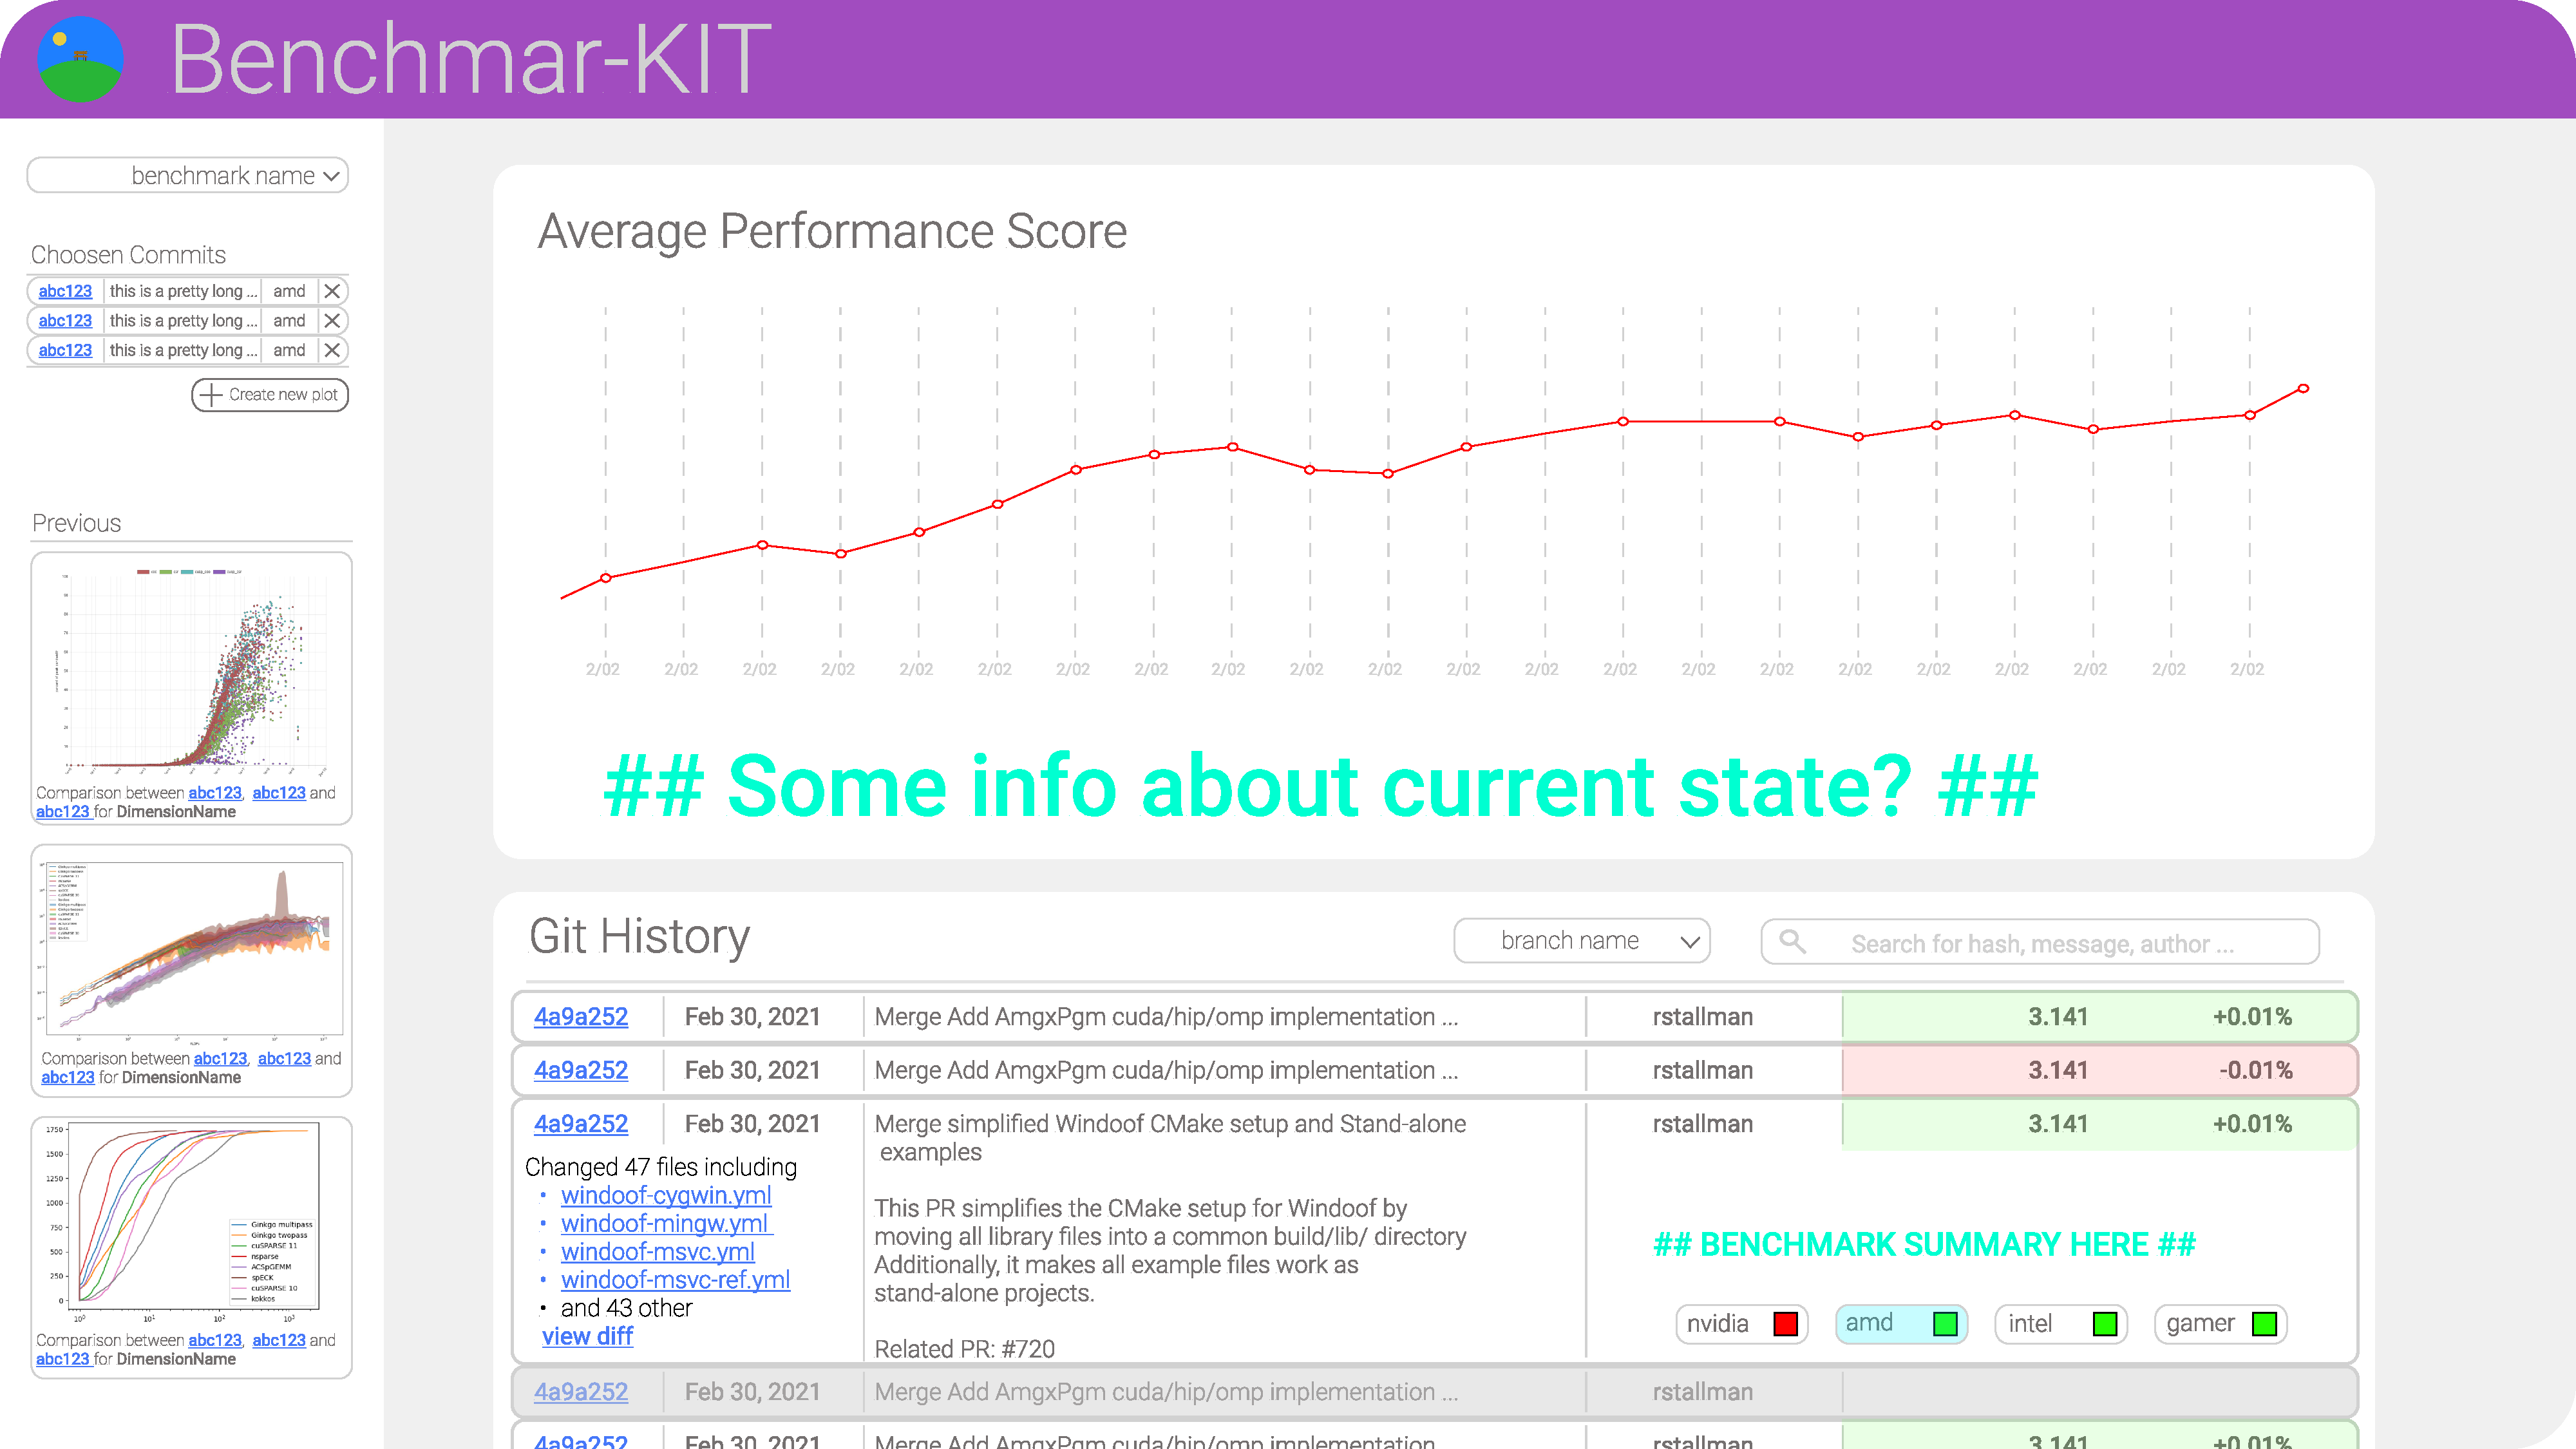
\includegraphics[width=\textwidth]{MainPage.pdf}
\captionof{figure}{Main page}

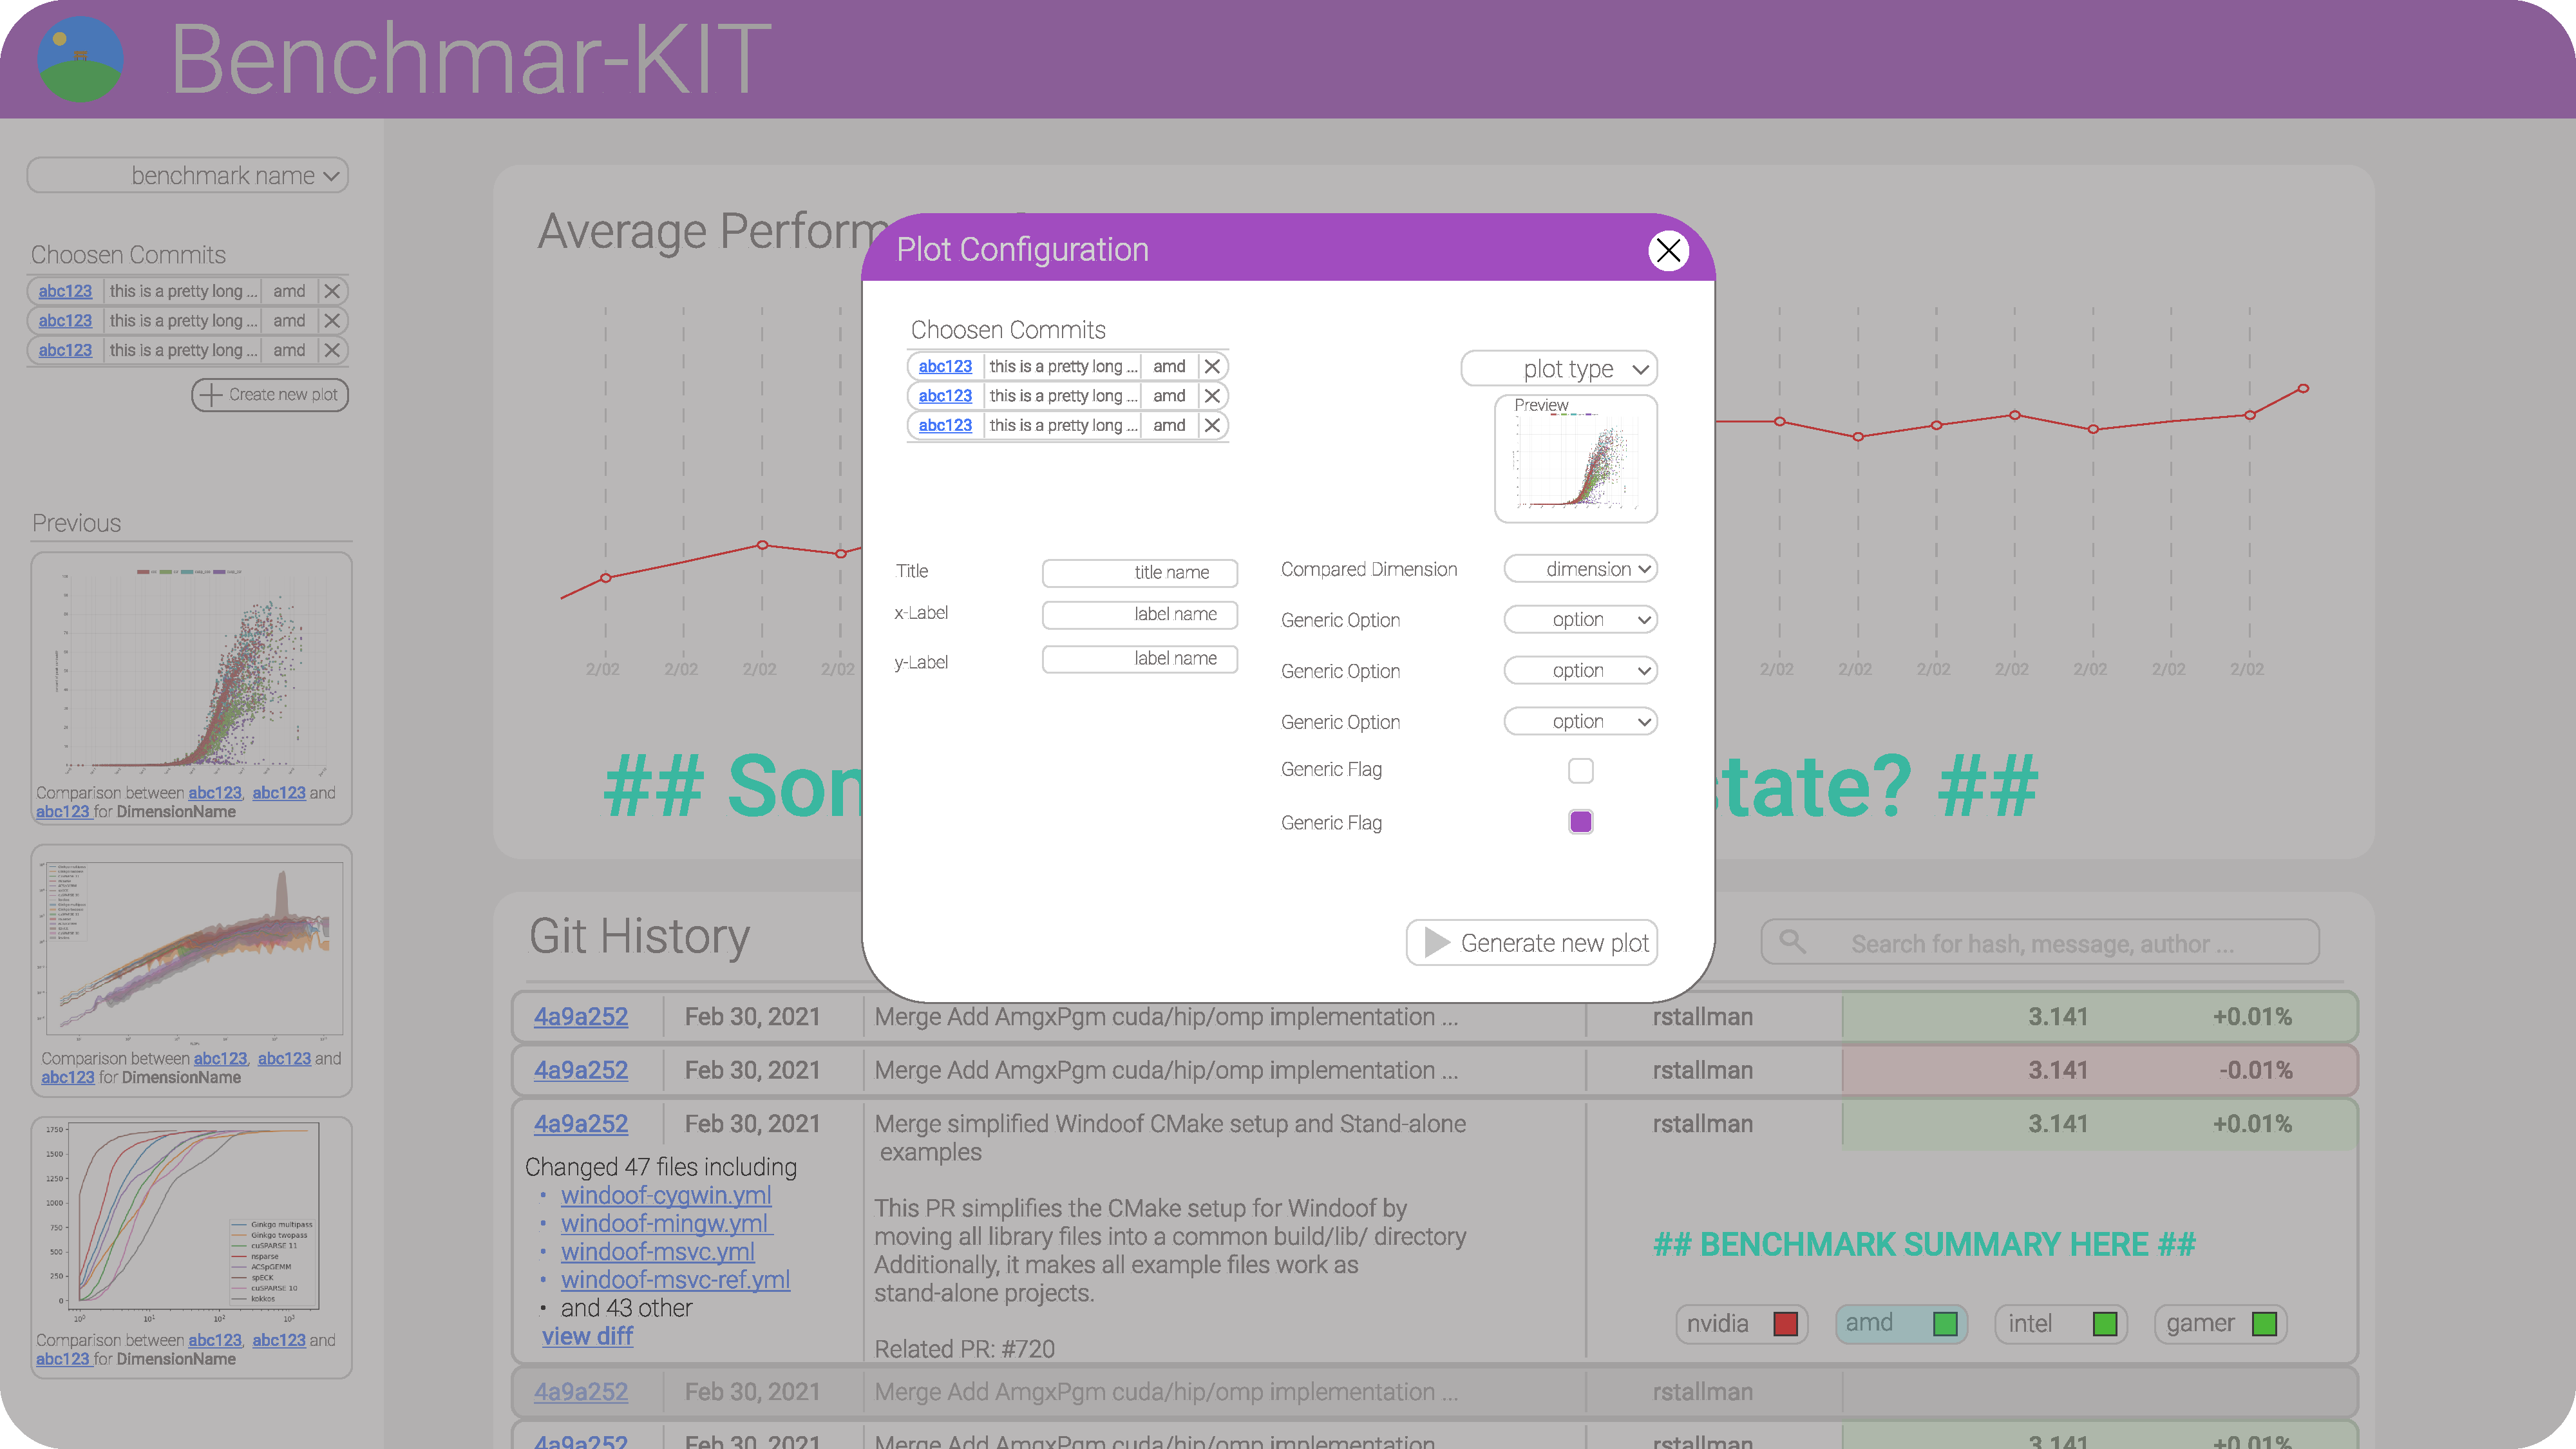
\includegraphics[width=\textwidth]{ConfigurationPopup.pdf}
\captionof{figure}{Configuration Popup}

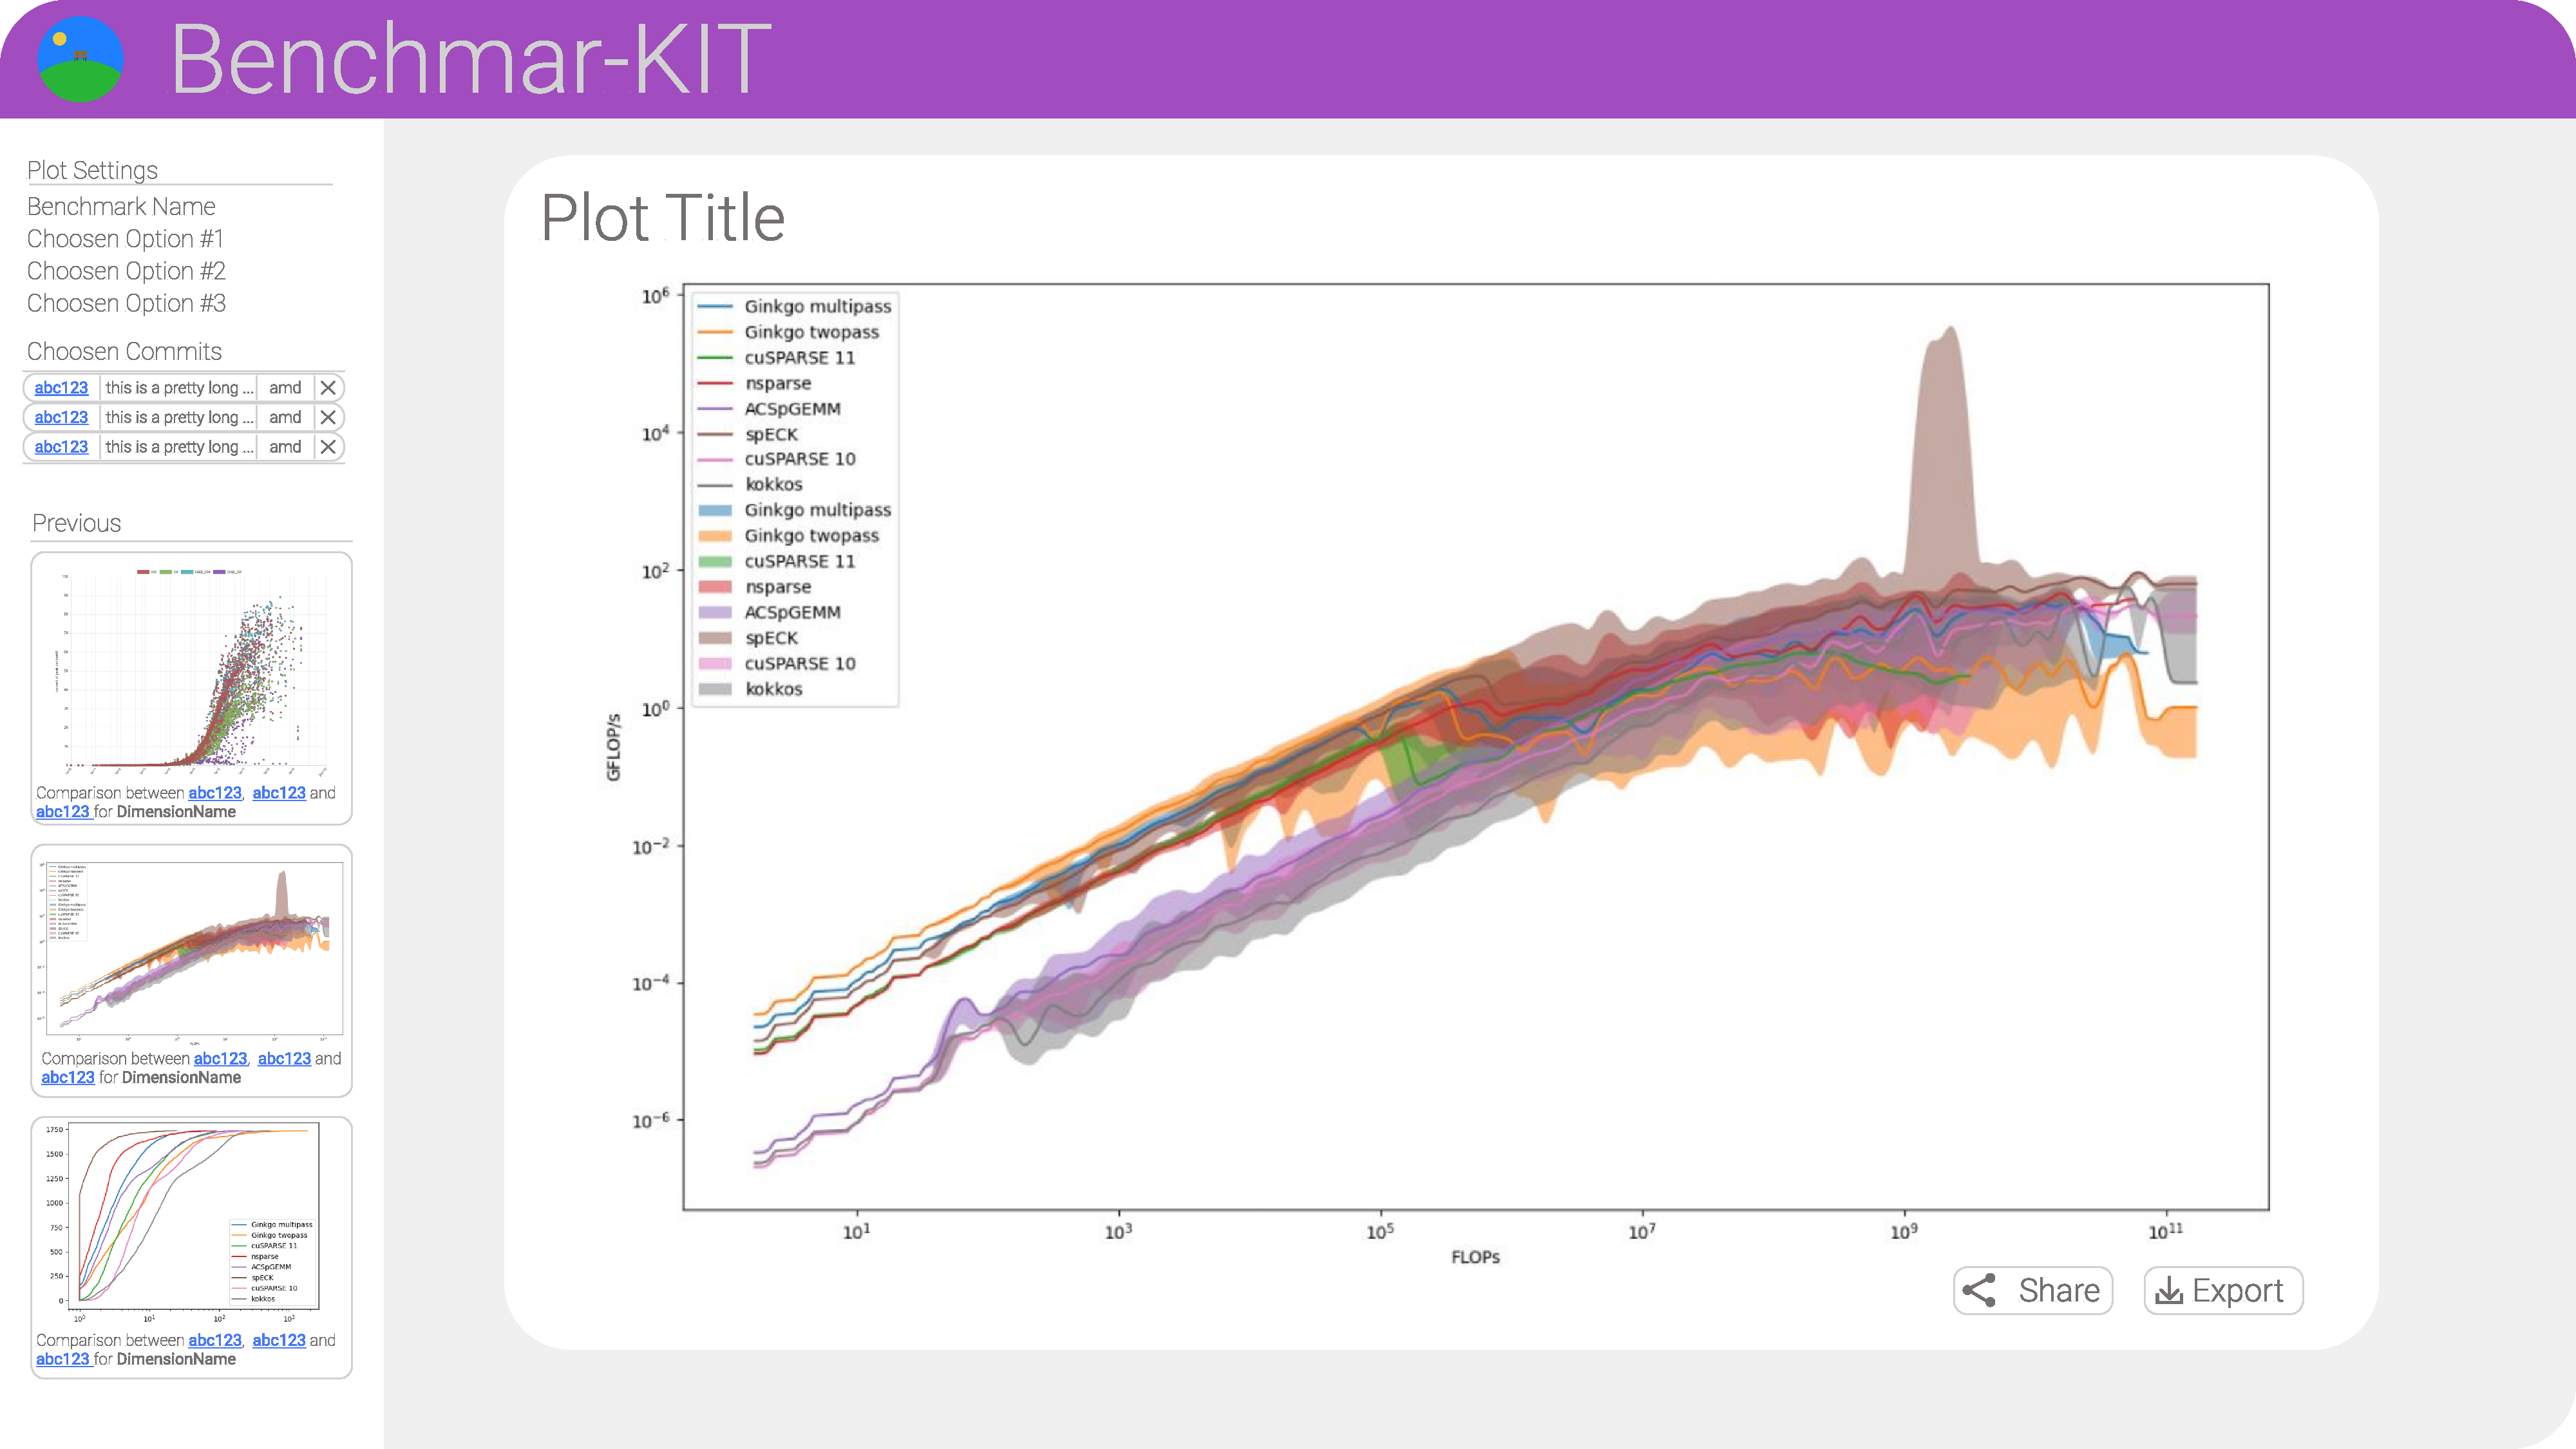
\includegraphics[width=\textwidth]{PlotView.pdf}
\captionof{figure}{View of a \gls{visualization}}

\clearpage

\section{Tests}

\test{Create Plot}{tst:create-vis-single}
\tests{fnc:select}
\tests{fnc:configure}
\tests{fnc:display}
\tests{fnc:overview}

Tests the basic navigation of the web app and the generation of a \gls{plot} from a set of datapoints.

\teststep{User has the web app open and no commits selected. The database contains \glspl{benchmark result}}
{User selects two commits}
{Commits get added to the list of selected commits}

\teststep{User has two commits selected}
{User selects the \enquote{Create New Plot} option}
{A popup with configuration options appears}

\teststep{User has two commits selected and the configuration popup open}
{User adjusts the configuration}
{Configuration gets updated on screen}

\teststep{User has two commits selected and the configuration popup open and has it configured}
{User selects the \enquote{Generate Plot} option}
{The \gls{plot} matching the configuration gets displayed to the user}

\test{Post Benchmark Results}{tst:post-data}
\tests{fnc:storage}

Tests sending \glspl{benchmark result} to the system and storing it.

\teststepnostate{The system receives a POST request with valid data}
{The data gets stored in the database}

\test{Error Handling}{tst:error}
\tests{nfc:robust}

Tests the system's ability to deal with malformed input data and invalid requests.

\teststep{Database is empty}
{System receives a POST request with malformed data for commit A}
{System does not store the data}

\teststep{Database is empty}
{The web app requests data for commit A}
{An error message gets displayed on the web app}

\test{Templates}{tst:template}
\tests{fnc:store-template}
\tests{fnc:load-template}

Tests the creation, storage and usage of templates.

\teststep{User has commits selected and the web app with the configuration popup open. Configuration has been changed from the default.}
{User selects the \enquote{Save Template} option}
{Template gets stored in cookies.}

\teststep{Template is stored in cookies.}
{User selects the \enquote{Load Template} option}
{Template gets applied to the current configuration}

\test{Share}{tst:share}
\tests{fnc:share-link}

Tests the sharing of \glspl{plot}.

\teststep{User has the web app with a \gls{plot} open}
{User selects the \enquote{Share} option}
{Link leads to a identical \gls{plot}}

\test{Export}{tst:export}
\tests{fnc:export}

Tests the export of \glspl{plot}.

\teststep{User has the web app with a \gls{plot} open}
{User selects the \enquote{Export} option}
{The \gls{plot} gets downloaded}

\test{Invalid Authentification}{tst:auth}
\tests{fnc:auth}

Tests the system ability to reject data without valid authentification 

\teststepnostate{The system receives a POST request with an invalid authentification}
{The system rejects the request and returns the corresponding error code}

\test{Performance Tracking}{tst:tracking}
\tests{fnc:calc}
\tests{fnc:track}
\tests{fnc:notify}

Tests the systems ability to detect performance drops and notify external webservices.

\teststep{The database contains a commit with high performance scores and a hook for an external webservice is set up}
{System gets a post request with data that has low performance scores}
{The external webserivce gets notified of the performance drop}

\clearpage

\section{Scenarios}

\scenario{Inspecting Last Change}{scn:inspect_last_change}
{Ted: \Gls{user}, CI: \Gls{benchmarking system}}
{Ted works on a project that has \emph{PROJECT NAME} set up. He makes changes on a performance critical component. After that he pushes his changes to the repository. The CI sends its benchmark results to the system, which stores it in a persistent way. Ted opens the webapp and selects a benchmark. He sees a list of all recent changes. The changes without benchmark data are greyed out. Ted selects his newest change. He selects a device to take the benchmark data from. The change appears in a list of selected changes. Ted selects the \enquote{Create New Plot} option. A popup appears. Ted chooses the dimension he wants to inspect. After he configured his plot he decides to save the \gls{template} for later use. He selects the \enquote{Save Template} option. He enters a name for the \gls{template} and selects the \enquote{Save} option. After that he selects the \enquote{Generate Plot} option. Ted gets redirected to a new site where he can inspect his plot. He decides to send this plot to a coworker. He selects the \enquote{Share} option and a link gets displayed. He copies the link and sends it to his coworker.}

\scenario{Comparing Benchmarks}{scn:comp_benchmarks}
{Greta: \Gls{user}}
{Greta opens the webapp. She selects a benchmark. She selects two benchmarks by first picking a specific change and then a specific device. She opens the configuration popup by selecting the \enquote{Create New Plot} option. She wants to use a previously created \gls{template}. She selects the \enquote{Use Template} option and chooses her \gls{template} from a list of available ones. The settings specified in the \gls{template} get applied to the current \gls{configuration}. Greta makes final adjustments and then selects the \enquote{Generate Plot} option. After that she gets redirected to a new site where she can inspect her plot. Ted also wants to download the plot for use in his publication. He selects the \enquote{Export} option. He gets to choose between a seleciton of filetypes. He picks his preferred one. A link gets displayed leading to a download with the selected filetype.}

\scenario{Performance Tracking}{scn:perf_tracking}
{CI: \Gls{benchmarking system}}
{The CI runs a specific benchmark for a specific change on a specific device. It sends a POST request to the system containing the results and the benchmark type, change identification and device name. The system receives the results and stores them in a persistent database. It recognizes that the benchmark performance has dropped by a significant factor. The system triggers a hook that sends a message to the developer slack channel informing about the performance drop. It also publishes a comment under the change on GitHub.}


\clearpage

\section{Use Cases}

\begin{figure}[H]
    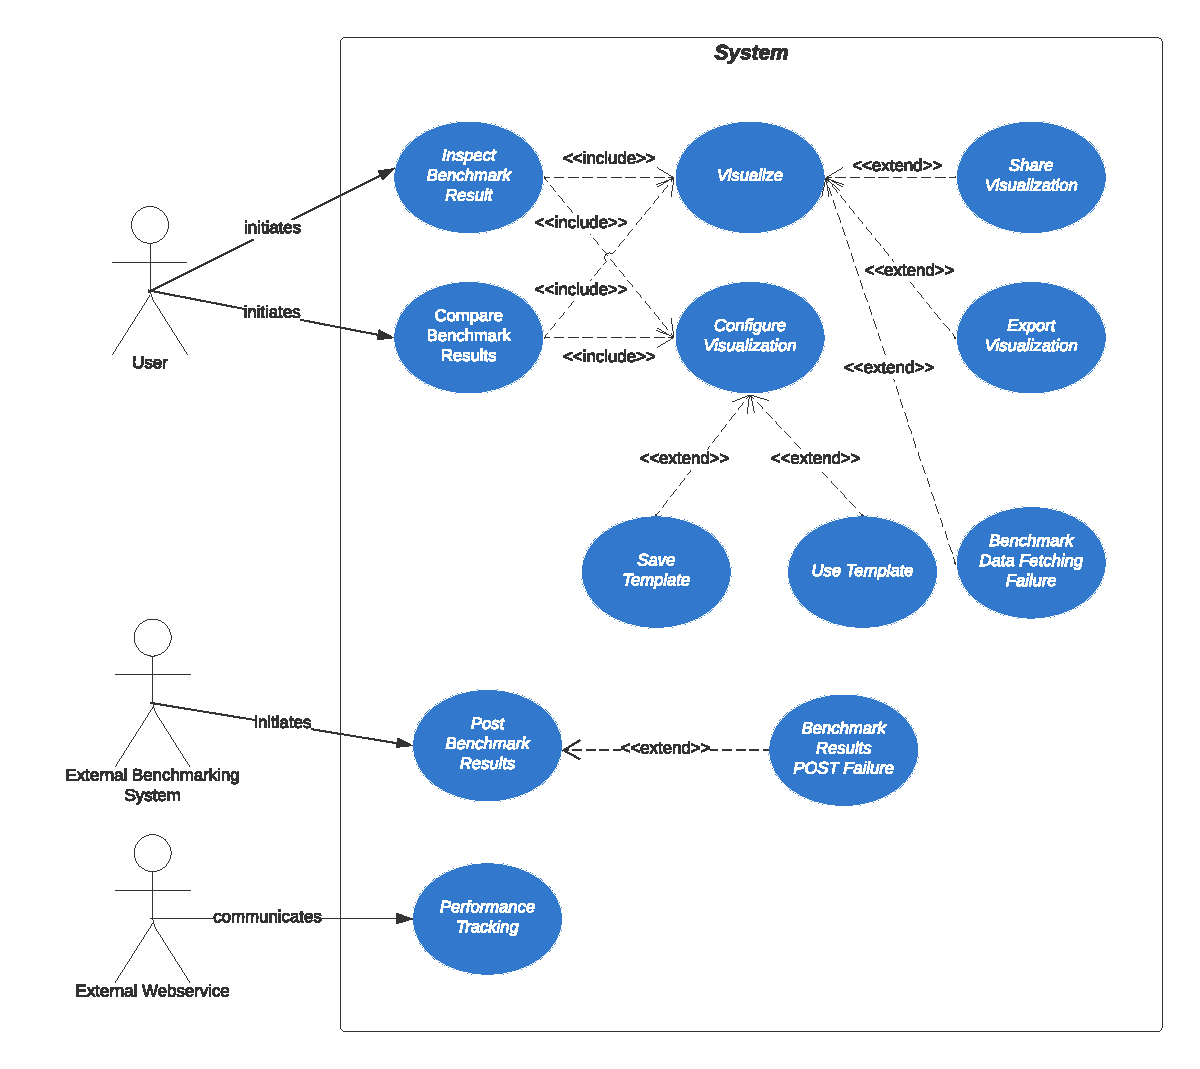
\includegraphics[width=\textwidth]{usecase.pdf}
    \caption{Use case diagram}
    \label{fig:usecase}
\end{figure}

\case{Plot}{cse:plot}
{Generating and displaying a Plot to a User}
{initiated by User}
{\gls{configuration} is available}
{\begin{enumerate}
    \item \parkview{} fetches a \gls{configuration} data from its database.
    \item \parkview{} takes the data and generates the plot specified in the \gls{configuration}.
    \item The user gets redirected to a new site where he can inspect the generated \gls{plot}.
\end{enumerate}}
{The plot specified by the \gls{configuration} gets shown to the User.}
\implementedby{scn:inspect-last-commit}{cse:plot}
\implementedby{scn:comp-benchmarks}{cse:plot}
\implementedby{scn:fetch-data-failure}{cse:plot}

\bigskip

\case{Configure Plot}{cse:config-vis}
{Configration of a \gls{plot}}
{initiated by User}
{User selected the \enquote{Create New Plot} option}
{\begin{enumerate}
    \item A popup appears.
    \item The user chooses a \gls{plot} type.
    \item The user chooses between certain options that are specific to the plot type, for example axis labels, plot title or compared dimensions.
\end{enumerate}}
{The \gls{configuration} gets updated.}
\implementedby{scn:inspect-last-commit}{cse:config-vis}
\implementedby{scn:comp-benchmarks}{cse:config-vis}
\implementedby{scn:fetch-data-failure}{cse:config-vis}

\bigskip

\case{Create New Plot}{cse:create-plot}
{Process for configuring and generating a plot}
{initated by User}
{benchmark data for commit is available}
{\begin{enumerate}
    \item The user selects a set of commits.
    \item The user initiates the \texttt{Configure Plot} use case by selecting the \enquote{Create New Plot} option.
    \item Once the user is satisfied with his \gls{configuration}, he initiates the \texttt{Plot} use case by selecting the \enquote{Create New Plot} option in the popup.
\end{enumerate}}
{Plot is displayed to the user}
\implementedby{scn:inspect-last-commit}{cse:create-plot}
\implementedby{scn:comp-benchmarks}{cse:create-plot}

\bigskip

\case{Share Plot}{cse:share-vis}
{Sharing a \gls{plot} using a link}
{initiated by User}
{A \gls{plot} has been generated}
{\begin{enumerate}
    \item The user selects the \enquote{Share Plot} option.
    \item A link gets displayed.
    \item The link redirects any visitors to the same \gls{plot}.
\end{enumerate}}
{A link is shown which redirects to the \gls{plot}}
\implementedby{scn:share}{cse:share-vis}

\bigskip

\case{Export Plot}{cse:export-vis}
{Downloading a plot}
{initiated by User}
{A \gls{plot} has been generated}
{\begin{enumerate}
    \item The user selects the \enquote{Export Plot} option.
    \item A popup appears.
    \item The user chooses a filetype for the export.
    \item The user confirms and downloads the \gls{plot} in the chosen file format.
\end{enumerate}}
{The User is offered a download of an export of the \gls{plot}}
\implementedby{scn:export}{cse:export-vis}

\bigskip

\case{Save Template}{cse:save-template}
{Storing a \gls{template} for later use}
{initiated by User}
{The user is in the \texttt{Configure Plot} use case}
{The \texttt{Save Template} use case extends the \texttt{Configure Plot} use case.
\begin{enumerate}
    \item The User selects the \enquote{save template} option.
    \item The User enters a name for the \gls{template}.
    \item The User gets a \gls{json} download for his \gls{template}.
    \item \parkview{} stores the template locally for the User (cookies).
\end{enumerate}}
{\Gls{template} is stored locally}
\implementedby{scn:template}{cse:save-template}

\bigskip

\case{Use Template}{cse:use-temp}
{Using a previously created template}
{initiated by User}
{The user is in the \texttt{Configure Plot} use case and a \gls{template} is available locally}
{The \texttt{Use Template} use case extends the \texttt{Configure Plot} use case.
\begin{enumerate}
    \item The User selects the \enquote{use template} option.
    \item User is shown a list of all available \glspl{template}.
    \item User selects a \gls{template} from the list.
    \item The current \gls{configuration} options get set to the values specified in the template.
\end{enumerate}}
{The \gls{template} is applied to the current configuration.}
\implementedby{scn:template}{cse:use-temp}

\bigskip

\case{Post Benchmark Results}{cse:post-benchmark-res}
{An external \gls{benchmarking system} trying to upload benchmark data}
{initiated by External Benchmarking System}
{The external \gls{benchmarking system} ran the benchmarks}
{\begin{enumerate}
    \item \parkview{} receives a POST request containing benchmark data.
    \item \parkview{} converts the received data into the correct format.
    \item \parkview{} stores the received data in its database.
\end{enumerate}}
{The received performance data is stored in the database}
\implementedby{scn:perf-tracking}{cse:post-benchmark-res}
\implementedby{scn:post-data-failure}{cse:post-benchmark-res}

\bigskip

\case{Performance Tracking}{cse:perf-tracking}
{\parkview{} recognizes big changes in performance and notifies external webservices}
{communicates with External Webservice}
{New benchmark data has been posted to the backend}
{\begin{enumerate}
    \item \parkview{} evaluates the performance of the new benchmark data.
    \item \parkview{} compares the performance of the new benchmark with the performance of the corresponding benchmark of the last commit.
    \item \parkview{} relays the results to a configured number of hooks.
    \item The hooks contact their external webservices according to how they have been configured.
\end{enumerate}}
{\parkview{} fires a POST Request to all webhook subscribers}
\implementedby{scn:perf-tracking}{cse:perf-tracking}

\bigskip

\case{Benchmark Results POST Failure}{cse:benchmark-res-post-fail}
{Behavior in case of invalid POST request}
{communicates with External \Gls{benchmarking system}}
{The external \gls{benchmarking system} has sent a POST request}
{This use case extends the \texttt{Post Benchmark Results} use case if an error occurs.
\begin{enumerate}
    \item \parkview{} identifies the error.
    \item \parkview{} creates a response with the correct error code.
\end{enumerate}}
{External Benchmarking System receives a response containing an error code}
\implementedby{scn:post-data-failure}{cse:benchmark-res-post-fail}

\bigskip

\case{Benchmark Data Fetching Failure}{cse:benchmark-data-fetch-fail}
{Behavior in case of invalid request for benchmark data}
{displays error to User}
{This use case extends the \texttt{Plot} use case if an error occurs.}
{\begin{enumerate}
    \item \parkview{} identifies the error.
    \item \parkview{} creates a response with the correct error code.
    \item \parkview{} app displays an error message in the browser.
\end{enumerate}}
{Error message gets displayed}
\implementedby{scn:fetch-data-failure}{cse:benchmark-data-fetch-fail}


\clearpage

\appendix

\printnoidxglossaries

\end{document}
